\part{Pixel Architecture}

\chapter{Subpixel Layouts}

\section{RGB Stripe Architecture}

\begin{figure}[H]
\centering
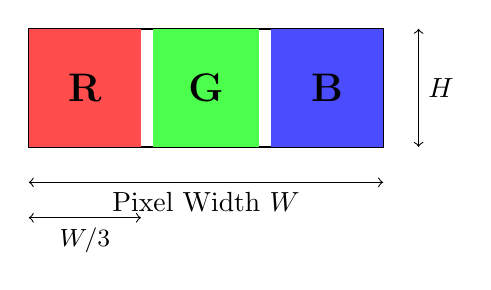
\begin{tikzpicture}[scale=1.5]
  % Draw pixel boundary
  \draw[thick] (0,0) rectangle (3,1);
  
  % RGB subpixels
  \fill[red!70] (0,0) rectangle (0.95,1);
  \fill[green!70] (1.05,0) rectangle (1.95,1);
  \fill[blue!70] (2.05,0) rectangle (3,1);
  
  % Labels
  \node at (0.475,0.5) {\Large\textbf{R}};
  \node at (1.5,0.5) {\Large\textbf{G}};
  \node at (2.525,0.5) {\Large\textbf{B}};
  
  % Dimensions
  \draw[<->] (0,-0.3) -- (3,-0.3) node[midway,below] {Pixel Width $W$};
  \draw[<->] (3.3,0) -- (3.3,1) node[midway,right] {$H$};
  \draw[<->] (0,-0.6) -- (0.95,-0.6) node[midway,below,font=\small] {$W/3$};
  
\end{tikzpicture}
\caption{RGB stripe subpixel layout. Three equal vertical stripes per pixel.}
\label{fig:rgb_stripe}
\end{figure}

\begin{formulabox}{RGB Stripe Geometry}
For pixel dimensions $W \times H$:
\begin{align}
  \text{Subpixel width} &= \frac{W}{3} \\
  \text{Subpixel height} &= H \\
  \text{Subpixel aspect ratio} &= \frac{H}{W/3} = \frac{3H}{W} \\
  \text{Total subpixels} &= 3WH \quad \text{(for $W \times H$ pixel display)}
\end{align}
\end{formulabox}

\subsection{Advantages and Disadvantages}

\begin{table}[H]
\centering
\caption{RGB Stripe Trade-offs}
\label{tab:rgb_tradeoffs}
\begin{tabular}{@{}p{6cm}p{6cm}@{}}
\toprule
\textcolor{successcolor}{\textbf{Advantages}} & \textcolor{accentcolor}{\textbf{Disadvantages}} \\
\midrule
Maximum horizontal resolution & Higher manufacturing cost \\
Optimal text rendering & Lower fill factor (60--70\%) \\
True color accuracy & Higher OLED power for white \\
No special rendering needed & PPI limited by FMM precision \\
Uniform aging & --- \\
\bottomrule
\end{tabular}
\end{table}

\section{PenTile Diamond Matrix}

\begin{figure}[H]
\centering
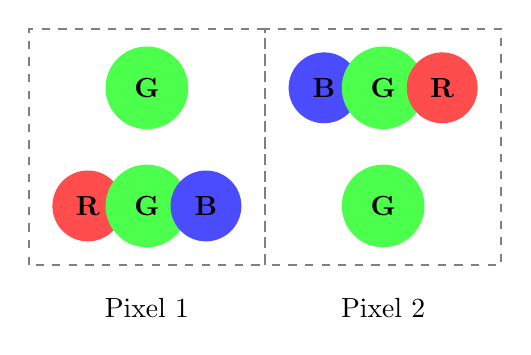
\begin{tikzpicture}[scale=1.5]
  % Draw two pixel boundaries
  \draw[thick,dashed,gray] (0,0) rectangle (2,2);
  \draw[thick,dashed,gray] (2,0) rectangle (4,2);
  
  % PenTile RGBG arrangement
  % First pixel
  \fill[red!70] (0.5,0.5) circle (0.3cm);
  \node at (0.5,0.5) {\textbf{R}};
  
  \fill[green!70] (1,1.5) circle (0.35cm);
  \node at (1,1.5) {\textbf{G}};
  
  \fill[green!70] (1,0.5) circle (0.35cm);
  \node at (1,0.5) {\textbf{G}};
  
  \fill[blue!70] (1.5,0.5) circle (0.3cm);
  \node at (1.5,0.5) {\textbf{B}};
  
  % Second pixel (shared subpixels)
  \fill[blue!70] (2.5,1.5) circle (0.3cm);
  \node at (2.5,1.5) {\textbf{B}};
  
  \fill[green!70] (3,1.5) circle (0.35cm);
  \node at (3,1.5) {\textbf{G}};
  
  \fill[green!70] (3,0.5) circle (0.35cm);
  \node at (3,0.5) {\textbf{G}};
  
  \fill[red!70] (3.5,1.5) circle (0.3cm);
  \node at (3.5,1.5) {\textbf{R}};
  
  % Labels
  \node[below] at (1,-0.2) {Pixel 1};
  \node[below] at (3,-0.2) {Pixel 2};
  
\end{tikzpicture}
\caption{PenTile diamond RGBG arrangement. Note how red and blue subpixels are shared between adjacent pixels.}
\label{fig:pentile}
\end{figure}

\begin{definitionbox}{PenTile Configuration}
PenTile RGBG uses:
\begin{itemize}
  \item 2 green subpixels per pixel (GG)
  \item 1 red subpixel shared between 2 horizontal pixels
  \item 1 blue subpixel shared between 2 horizontal pixels
\end{itemize}

\textbf{Effective subpixel count:}
\begin{equation}
  N_{\text{subpixels}} = 2N_{\text{pixels}}
\end{equation}
Compare to RGB stripe: $3N_{\text{pixels}}$

This represents a 33\% reduction in physical subpixels.
\end{definitionbox}

\subsection{Theoretical Foundation}

PenTile exploits two psychovisual properties:

\begin{enumerate}
  \item \textbf{Higher green sensitivity:} M-cone density approximately 2× L-cone density
  \item \textbf{Luminance dominance:} Spatial resolution determined primarily by luminance channel (green contributes ~70\% to luminance)
\end{enumerate}

\begin{formulabox}{Effective PenTile Resolution}
For PenTile display with stated resolution $N \times M$:
\begin{align}
  R_{\text{eff,horizontal}} &\approx 0.71 \times N_{\text{stated}} \\
  R_{\text{eff,vertical}} &\approx M_{\text{stated}}
\end{align}

The 0.71 factor ($\sqrt{0.5}$) arises from the checkerboard arrangement of red and blue subpixels.
\end{formulabox}

\begin{examplebox}{Example: Samsung Galaxy S24}
Stated resolution: 3088 × 1440 pixels (PenTile)

Effective resolution:
\begin{itemize}
  \item Horizontal: $3088 \times 0.71 \approx 2192$ equivalent RGB pixels
  \item Vertical: $1440$ pixels (unchanged)
\end{itemize}

Comparable to RGB stripe display: $2192 \times 1440$

However, the stated 3088 × 1440 sounds better for marketing!
\end{examplebox}

\section{RGBW Configuration}

\begin{figure}[H]
\centering
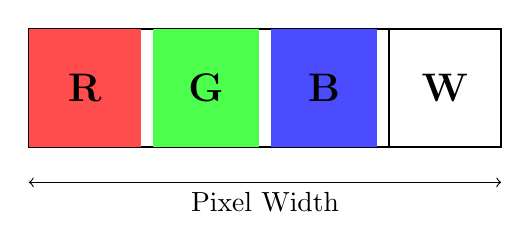
\begin{tikzpicture}[scale=1.5]
  % Draw pixel boundary
  \draw[thick] (0,0) rectangle (4,1);
  
  % RGBW subpixels
  \fill[red!70] (0,0) rectangle (0.95,1);
  \fill[green!70] (1.05,0) rectangle (1.95,1);
  \fill[blue!70] (2.05,0) rectangle (2.95,1);
  \fill[white] (3.05,0) rectangle (4,1);
  \draw[thick] (3.05,0) rectangle (4,1); % Border for white
  
  % Labels
  \node at (0.475,0.5) {\Large\textbf{R}};
  \node at (1.5,0.5) {\Large\textbf{G}};
  \node at (2.5,0.5) {\Large\textbf{B}};
  \node at (3.525,0.5) {\Large\textbf{W}};
  
  % Dimensions
  \draw[<->] (0,-0.3) -- (4,-0.3) node[midway,below] {Pixel Width};
  
\end{tikzpicture}
\caption{RGBW subpixel layout with white subpixel for improved power efficiency.}
\label{fig:rgbw}
\end{figure}

\begin{formulabox}{RGBW Conversion Algorithm}
To convert RGB input to RGBW output:
\begin{align}
  W &= \min(R, G, B) \\
  R' &= R - W \\
  G' &= G - W \\
  B' &= B - W
\end{align}

\textbf{Power efficiency for full white:}
\begin{itemize}
  \item RGB stripe OLED: 3 subpixels active
  \item RGBW OLED: 1 subpixel active (white is more efficient)
  \item Power savings: Approximately 3--4× for white content
\end{itemize}
\end{formulabox}

\begin{table}[H]
\centering
\caption{Subpixel Layout Comparison}
\label{tab:subpixel_comparison}
\begin{tabular}{@{}lcccc@{}}
\toprule
\textbf{Property} & \textbf{RGB Stripe} & \textbf{PenTile} & \textbf{RGBW} \\
\midrule
Subpixels/pixel & 3 & 2 & 4 \\
Text clarity & Excellent & Good & Fair \\
Power efficiency & Baseline & +33\% & +200--300\% \\
Color gamut & Full & Full & Reduced \\
Manufacturing & Complex & Medium & Complex \\
Cost & High & Medium & High \\
\bottomrule
\end{tabular}
\end{table}

% ============================================================================
% PART III: GAMMA AND TRANSFER FUNCTIONS
% ============================================================================

